%Author Alex Clemmer
%CS 3810 Computer Organization
%Assignment1:
\documentclass[a4paper]{article}
\usepackage[pdftex]{graphicx}
\usepackage{fancyvrb}
\usepackage{multirow}
\usepackage{amssymb}

\begin{document}

\section*{Assignment 1 }
Author: Alex Clemmer\\
Student number: u0458675

\subsection*{Problem 1:}
\paragraph*{1.3.1:} The clear winner is P2. The rightmost column is the result of the performance function (the middle column):

\begin{center}
\begin{tabular}{|c|c|c|c|c|}
\hline
Processor & \multicolumn{2}{|c|}{Performance Function} & \multicolumn{2}{|c|}{Performance}\\
\hline
P1 & \multicolumn{2}{|c|}{I $\times$ 200 ps $\times$ 1.5 CPI} & \multicolumn{2}{|c|}{400 $\cdot$ I ps}\\
\hline
P2 & \multicolumn{2}{|c|}{I $\times$ 150 ps $\times$ 1.0 CPI} & \multicolumn{2}{|c|}{150 $\cdot$ I ps}\\
\hline
P3 & \multicolumn{2}{|c|}{I $\times$ 300 ps $\times$ 2.5 CPI} & \multicolumn{2}{|c|}{750 $\cdot$ I ps}\\
\hline
\end{tabular}
\end{center}

\paragraph*{1.3.2:} If P1 takes 10 seconds to execute a job, and its clock speed is 2 GHz, then our clock speed is equal to the number of instructions executed in a second times the number of seconds, or: $2\times10^9 \times 10 =  2\times10^{10}$ cycles. Similarly, for P2, $1.5\times10^9 \times 10 = 1.5\times10^{10}$ cycles, and for P3, $3\times10^9 \times 10 = 3\times10^{10}$ cycles.

Given the total cycles, we can also calculate the instructions using the formula $\frac{\mbox{total cycles}}{\mbox{cycles per instruction}} = \mbox{instructions}$. That means P1$_{instr}$ = $\frac{2\times10^{10} cycles}{1.5 CPI}$, P2$_{instr}$ = $\frac{1.5\times10^{10} cycles}{1.0 CPI}$, and P3$_{instr}$ = $\frac{3\times10^{10} cycles}{2.5 CPI}$, which is all summarized by the third column of this chart:
\begin{center}
\begin{tabular}{|c|c|c|c|c|}
\hline
\multicolumn{5}{|c|}{Clock Cycles and total instructions given 10-second execution time}\\
\hline
\hline
Processor & \multicolumn{2}{|c|}{Cycles} & \multicolumn{2}{|c|}{Total Instructions Executed}\\
\hline
P1 & \multicolumn{2}{|c|}{$2\times10^{10}$ cycles} & \multicolumn{2}{|c|}{$1.333...\times10^{10}$ instructions}\\
\hline
P2 & \multicolumn{2}{|c|}{$1.5\times10^{10}$ cycles} & \multicolumn{2}{|c|}{$1.5\times10^{10}$ instructions}\\
\hline
P3 & \multicolumn{2}{|c|}{$3\times10^{10}$ cycles} & \multicolumn{2}{|c|}{$1.2\times10^{10}$ instructions}\\
\hline
\end{tabular}
\end{center}

\paragraph*{1.3.3:} ERROR: NOT DONE YET.

\subsection*{Problem 2:}

\paragraph*{1.11.1:} To calculate yield, we must first find the die area. For (a): 90 $\mbox{dies per wafer} = \frac{\mbox{wafer area}}{\mbox{die area}} = \frac{(\frac{15}{2})^2\pi}{\mbox{die area}_{(a)}}; \therefore \mbox{die area}_{(a)} = \frac{5\pi}{8}$. For (b): $140\mbox{ dies per wafer} = \frac{(\frac{25}{2})^2\pi}{\mbox{die area}_{(b)}}; \therefore \mbox{ die area}_{(b)} = \frac{125\pi}{112}$.

So the yield will be as follows:

\begin{equation}
\mbox{Yield}_{(a)} = \frac{1}{(1+.018 \frac{\frac{5\pi}{8}}{2})^2} \approx{.965572}
\end{equation}

\begin{equation}
\mbox{Yield}_{(b)} = \frac{1}{(1+.024 \frac{\frac{125\pi}{112}}{2})^2} \approx{.92087}
\end{equation}

\paragraph*{1.11.2:} Cost per die = $\frac{\mbox{cost per wafer}}{\mbox{dies per wafer} \times \mbox{yield}}$, so the operations are pretty straightforward:

\begin{equation}
\mbox{Cost per die}_{(a)} = \frac{10}{90 \cdot .96557} \approx{.115073}
\end{equation}

\begin{equation}
\mbox{Cost per die}_{(b)} = \frac{20}{140 \cdot .92087} \approx{.155131}
\end{equation}

\paragraph*{1.11.3:} Given a 10\% increase in dies per wafer, (a) now has 99 DPW and (b) now has 154 DPW. So our die area (using the formula from 1.11.1) will look like so:

\begin{equation}
99\mbox{ dies per wafer} = \frac{(\frac{15}{2})^2 \pi}{\mbox{die area}_{(a)}}; \therefore \mbox{die area}_{(a)} = \frac{25 \pi}{44}
\end{equation}

\begin{equation}
154\mbox{ dies per wafer} = \frac{(\frac{25}{2})^2 \pi}{\mbox{die area}_{(b)}}; \therefore \mbox{die area}_{(a)} = \frac{625 \pi}{616}
\end{equation}

Given a 15\% increase in defects per area, (a) is now at .0207 DPA, while (b) is now at .0276 DPA. 

\begin{equation}
\mbox{New Yield}_{(a)} = \frac{1}{(1+.018 \frac{\frac{5\pi}{8}}{2})^2} \approx{.96405}
\end{equation}

\begin{equation}
\mbox{New Yield}_{(b)} = \frac{1}{(1+.024 \frac{\frac{125\pi}{112}}{2})^2} \approx{.917507}
\end{equation}

\subsection*{Problem 3:}
\paragraph*{1.10.1:} We can calculate the number of instructions required for a job by adding up the number of instructions from each sub-set of the work (e.g., instructions = arithmetic + branch + load/store).

\begin{center}
\begin{tabular}{|c|c|c|c|c|c|}
\hline
& Total Processors & \multicolumn{2}{|c|}{Total Instruction Count} & \multicolumn{2}{|c|}{Aggregated Instruction Count}\\
\hline
\multirow{4}{*}{a} & 1 & \multicolumn{2}{|c|}{2560 + 1280 + 256 = {\bf4096}} & \multicolumn{2}{|c|}{$4096 \cdot 1 = {\bf4096}$}\\
& 2 & \multicolumn{2}{|c|}{1280 + 640 + 128 = {\bf2048}} & \multicolumn{2}{|c|}{$2048 \cdot 2 = {\bf4096}$}\\
& 4 & \multicolumn{2}{|c|}{640 + 320 + 64 = {\bf1024}} & \multicolumn{2}{|c|}{$1024 \cdot 4 = {\bf4096}$}\\
& 8 & \multicolumn{2}{|c|}{320 + 160 + 32 = {\bf512}} & \multicolumn{2}{|c|}{$512 \cdot 4 = {\bf4096}$}\\
\hline
\hline
\multirow{4}{*}{b} & 1 & \multicolumn{2}{|c|}{2560 + 1280 + 256 = {\bf4096}} & \multicolumn{2}{|c|}{$4096 \cdot 1 = {\bf4096}$}\\
& 2 & \multicolumn{2}{|c|}{1350 + 8000 + 128 = {\bf2278}} & \multicolumn{2}{|c|}{$2278 \cdot 2 = {\bf4556}$}\\
& 4 & \multicolumn{2}{|c|}{800 + 600 + 64 = {\bf1464}} & \multicolumn{2}{|c|}{$1464 \cdot 4 = {\bf5856}$}\\
& 8 & \multicolumn{2}{|c|}{600 + 500 + 32 = {\bf1132}} & \multicolumn{2}{|c|}{$1132 \cdot 4 = {\bf9056}$}\\
\hline
\end{tabular}
\end{center}

\paragraph*{1.10.2:} We can obtain the execution time by multiplying the cycles per instruction by the time it takes to execute one clock cycle: $\frac{1}{\mbox{length of cycle}} \cdot \mbox{CPI}$, where $\textit{length of cycle}$ = 2 $\cdot 10^9$ seconds. Thus, 

\begin{center}
\begin{tabular}{|c|c|c|c|c|c|}
\hline
& Total Processors & \multicolumn{2}{|c|}{Total Execution Time}\\
\hline
\multirow{4}{*}{a} & 1 & \multicolumn{2}{|c|}{$\frac{1}{781250} + \frac{1}{390625} + \frac{1}{3906250} \approx .000004$}\\
& 2 & \multicolumn{2}{|c|}{$\frac{1}{1562500} + \frac{1}{781250} + \frac{1}{7812500} \approx .000002$}\\
& 4 & \multicolumn{2}{|c|}{$\frac{1}{3125000} + \frac{1}{1562500} + \frac{1}{15625000} \approx .000001$}\\
& 8 & \multicolumn{2}{|c|}{$\frac{1}{6250000} + \frac{1}{3125000} + \frac{1}{31250000} \approx 3.2\times10^{-8}$}\\
\hline
\hline
\multirow{4}{*}{b} & 1 & \multicolumn{2}{|c|}{$\frac{1}{781250} + \frac{429}{50000000} + \frac{1}{3906250} \approx .000004$}\\
& 2 & \multicolumn{2}{|c|}{$\frac{27}{40000000} + \frac{3}{1250000} + \frac{1}{7812500} \approx .000003203$}\\
& 4 & \multicolumn{2}{|c|}{$\frac{1}{2500000} + \frac{27}{10000000} + \frac{1}{15625000} \approx .000003164$}\\
& 8 & \multicolumn{2}{|c|}{$\frac{3}{10000000} + \frac{13}{4000000} + \frac{1}{31250000} \approx .000003582$}\\
\hline
\end{tabular}
\end{center}

\paragraph*{1.10.3:} What happens when we double the arithmetic instructions? Let's find out:

\begin{center}
\begin{tabular}{|c|c|c|c|c|c|}
\hline
\multicolumn{4}{|c|}{Execution Time with Doubled Arithmetic Instructions}\\
\hline
\hline
& Total Processors & \multicolumn{2}{|c|}{Total Execution Time}\\
\hline
\multirow{4}{*}{b} & 1 & \multicolumn{2}{|c|}{$\frac{1}{390625} + \frac{429}{50000000} + \frac{1}{3906250} \approx .000005396$}\\
& 2 & \multicolumn{2}{|c|}{$\frac{27}{20000000} + \frac{3}{1250000} + \frac{1}{7812500} \approx .000003878$}\\
& 4 & \multicolumn{2}{|c|}{$\frac{1}{1250000} + \frac{27}{10000000} + \frac{1}{15625000} \approx .000003564$}\\
& 8 & \multicolumn{2}{|c|}{$\frac{3}{10000000} + \frac{13}{4000000} + \frac{1}{31250000} \approx .000003582$}\\
\hline
\end{tabular}
\end{center}

So when we compare the total execution time of this chart and the one from 1.10.2, we see that doubling the instruction count actually does cause a spike in execution time, at least in single-processor settings. But this disadvantage drops off precipitously as the number of processors goes up, which is what we would expect.

\subsection*{Problem 4:}


\paragraph*{Usage:}
I have included a trace which includes which provides all commands needed to test the facts, provided CLIPS is started and as2part1.clp is put into the same directory. In short, you clear out all old facts (this can be unnecessary if CLIPS was just started), we watch all facts that are inferred, then load then file, reset and finally run the rules. The result can be seen below.
\begin{Verbatim}[fontsize=\small]
CLIPS> (clear)
CLIPS> (watch facts)
CLIPS> (load as2part1.clp)
Defining deftemplate: animal
Defining defrule: animalfacts +j
Defining deftemplate: fish
Defining deftemplate: bird
Defining deftemplate: mammal
Defining defrule: fishisanimal +j
Defining defrule: birdisanimal +j
Defining defrule: mammalisanimal +j
Defining deffacts: starting-fish
Defining deffacts: starting-birds
Defining defrule: canfly +j
Defining defrule: canarycolour +j
Defining defrule: is-dangerous +j
Defining defrule: delicacy-is-eatable +j
TRUE
CLIPS> (reset)==> f-0     (initial-fact)
==> f-1     (fish (name shark) (has-gills TRUE) (can-swim TRUE) 
                  (lay-eggs FALSE) (attribs dangerous))
==> f-2     (fish (name salmon) (has-gills TRUE) (can-swim TRUE) 
                  (lay-eggs TRUE) (attribs delicacy))
==> f-3     (bird (name canary) (has-wings TRUE) (can-fly TRUE) 
                  (lay-eggs TRUE) (colour "yellow") (attribs))
==> f-4     (bird (name ostrich) (has-wings TRUE) (can-fly FALSE) 
                  (lay-eggs TRUE) (colour "Unknown") 
                  (attribs is-tall walks))
CLIPS> (run)
==> f-5     (animal (name ostrich))
==> f-6     (has-skin ostrich)
==> f-7     (animal (name canary))
==> f-8     (has-skin canary)
==> f-9     (flies canary)
==> f-10    (canarycolour "yellow")
==> f-11    (animal (name salmon))
==> f-12    (has-skin salmon)
==> f-13    (eatable salmon)
==> f-14    (animal (name shark))
==> f-15    (has-skin shark)
==> f-16    (isdangerous shark)
CLIPS> \end{Verbatim}
Below are the questions stated again for convenience, followed by the set of answers. \\ \textbf{Questions:}
\begin{itemize}
	\item 1. Can canaries fly??
	\item 2. What is the color of canaries??
	\item 3. Can ostriches fly??
	\item 4. Do canaries have skin??
	\item 5. Are sharks dangerous??
	\item 6. Can you eat salmon??
\end{itemize}
\textbf{Answers:}
\begin{itemize}
	\item 1. Yes, see f-9 (flies canary).
	\item 2. Yellow, see f-10 (canarycolour "yellow").
	\item 3. No, there is no fact (flies ostrich).
	\item 4. Yes, see f-8 (has-skin canary).
	\item 5. Yes, see f-16 (isdangerous shark).
	\item 6. Yes, see f-11 (eatable salmon).
\end{itemize}

\subsection*{2: Rule-based systems modeling and programming}
First we identify the conditions and values.  The conditions are the wealth (poor or rich), the age ($<25$ or $>=25$). The wealth conditions (rich or poor) need to be determined by the amount of earnings ($>100.000 euro$ or $<100.000 euro$) or savings ($>50.000 euro$ or $<50.000 euro$). Furthermore the wealth of the parents should also be a condition (in case the age is $<25$). So the conditions are: wealth, age, wealth of parents. These conditions depend on: earnings and savings. The actions taken are: LEC, no LEC (and possibly support by parents).  

\subsubsection*{a.}
First we put all the standard conditions in a table and after that we give a table for the conditions wealth depends on (earnings and savings).
\begin{center}
\begin{tabular}{|c|c|c|c|c|c|c|c|c|}
\hline
Wealth & \multicolumn{4}{|c|}{Rich} & \multicolumn{4}{|c|}{Poor}\\
\hline
Age & \multicolumn{2}{|c|}{$<25$} & \multicolumn{2}{|c|}{$>=25$} & \multicolumn{2}{|c|}{$<25$} & \multicolumn{2}{|c|}{$>=25$}\\
\hline
Wealth of parents & Rich & Poor & Rich & Poor & Rich & Poor & Rich & Poor\\
\hline
\hline
LEC granted & No & No & No & No & No & Yes & Yes & Yes \\
\hline
\end{tabular}
\end{center}
This table can of course be simplified.
\begin{flushleft}
\begin{tabular}{|c|c|c|c|c|c|c|c|c|}
\hline
Wealth & \multicolumn{4}{|c|}{Rich} & \multicolumn{4}{|c|}{Poor}\\
\hline
Age & \multicolumn{4}{|c|}{$-$} & \multicolumn{2}{|c|}{$<25$} & \multicolumn{2}{|c|}{$>=25$}\\
\hline
Wealth of parents & \multicolumn{4}{|c|}{$-$} & Rich & Poor &\multicolumn{2}{|c|}{-}\\
\hline
LEC granted & \multicolumn{4}{|c|}{No} & No & Yes & \multicolumn{2}{|c|}{Yes} \\
\hline
\end{tabular}
\end{flushleft}
Now to specify the table for when condition wealth holds.
\begin{flushleft}
\begin{tabular}{|c|c|c|c|c|}
\hline
Earnings & \multicolumn{2}{|c|}{$>100.000$} & \multicolumn{2}{|c|}{$<=100.000$}\\
\hline
Savings & $>50.000$ & $<=50.000$ & $>50.000$ & $<=50.000$\\
\hline
Rich & Yes & Yes & Yes & No\\
\hline
\end{tabular}
\end{flushleft}
This table can also be simplified.
\begin{flushleft}
\begin{tabular}{|c|c|c|c|c|}
\hline
Earnings & \multicolumn{2}{|c|}{$>100.000$} & \multicolumn{2}{|c|}{$<=100.000$}\\
\hline
Savings & \multicolumn{2}{|c|}{-} & $>50.000$ & $<=50.000$\\
\hline
Rich & \multicolumn{2}{|c|}{Yes} & Yes & No\\
\hline
\end{tabular}
\end{flushleft}
So we will need a total of $4 + 3 = 7$ rules.

\subsubsection*{b.}
See the attached CLIPS file as2part2.clp for the rules implementing the decision tables. Now we give two example traces of our CLIPS implementation of the tables. First a trace of a person who has high earnings (and thus gets no LEC). Followed by  a trace of a person with low savings, low earnings, age less than 25, and poor parents (and thus gets LEC).
\begin{Verbatim}[fontsize=\small]
CLIPS> (clear)
CLIPS> (watch facts)
CLIPS> (load as2part2.clp)
Defining defrule: rich_rule1 +j
Defining defrule: rich_rule2 +j+j
Defining defrule: rich_rule3 =j+j
Defining defrule: lec_rule1 +j
Defining defrule: lec_rule2 +j+j+j
Defining defrule: lec_rule3 =j=j+j
Defining defrule: lec_rule4 =j+j
TRUE
CLIPS> (assert (earnings 123456789))
==> f-0     (earnings 123456789)
<Fact-0>
CLIPS> (run)
==> f-1     (wealth rich)
==> f-2     (LEC not_granted)
\end{Verbatim}
\begin{Verbatim}[fontsize=\small]
CLIPS> (clear)
CLIPS> (watch facts)
CLIPS> (load as2part2.clp)
Defining defrule: rich_rule1 +j
Defining defrule: rich_rule2 +j+j
Defining defrule: rich_rule3 =j+j
Defining defrule: lec_rule1 +j
Defining defrule: lec_rule2 +j+j+j
Defining defrule: lec_rule3 =j=j+j
Defining defrule: lec_rule4 =j+j
TRUE
CLIPS> (assert (earnings 10000))
==> f-0     (earnings 10000)
<Fact-0>
CLIPS> (assert (savings 100))
==> f-1     (savings 100)
<Fact-1>
CLIPS> (assert (age 10))
==> f-2     (age 10)
<Fact-2>
CLIPS> (assert (wealth_parents poor))
==> f-3     (wealth_parents poor)
<Fact-3>
CLIPS> (run)
==> f-4     (wealth poor)
==> f-5     (LEC granted)
\end{Verbatim}

\subsection*{3: Programming in CLIPS}

\begin{figure}[htp]
\centering
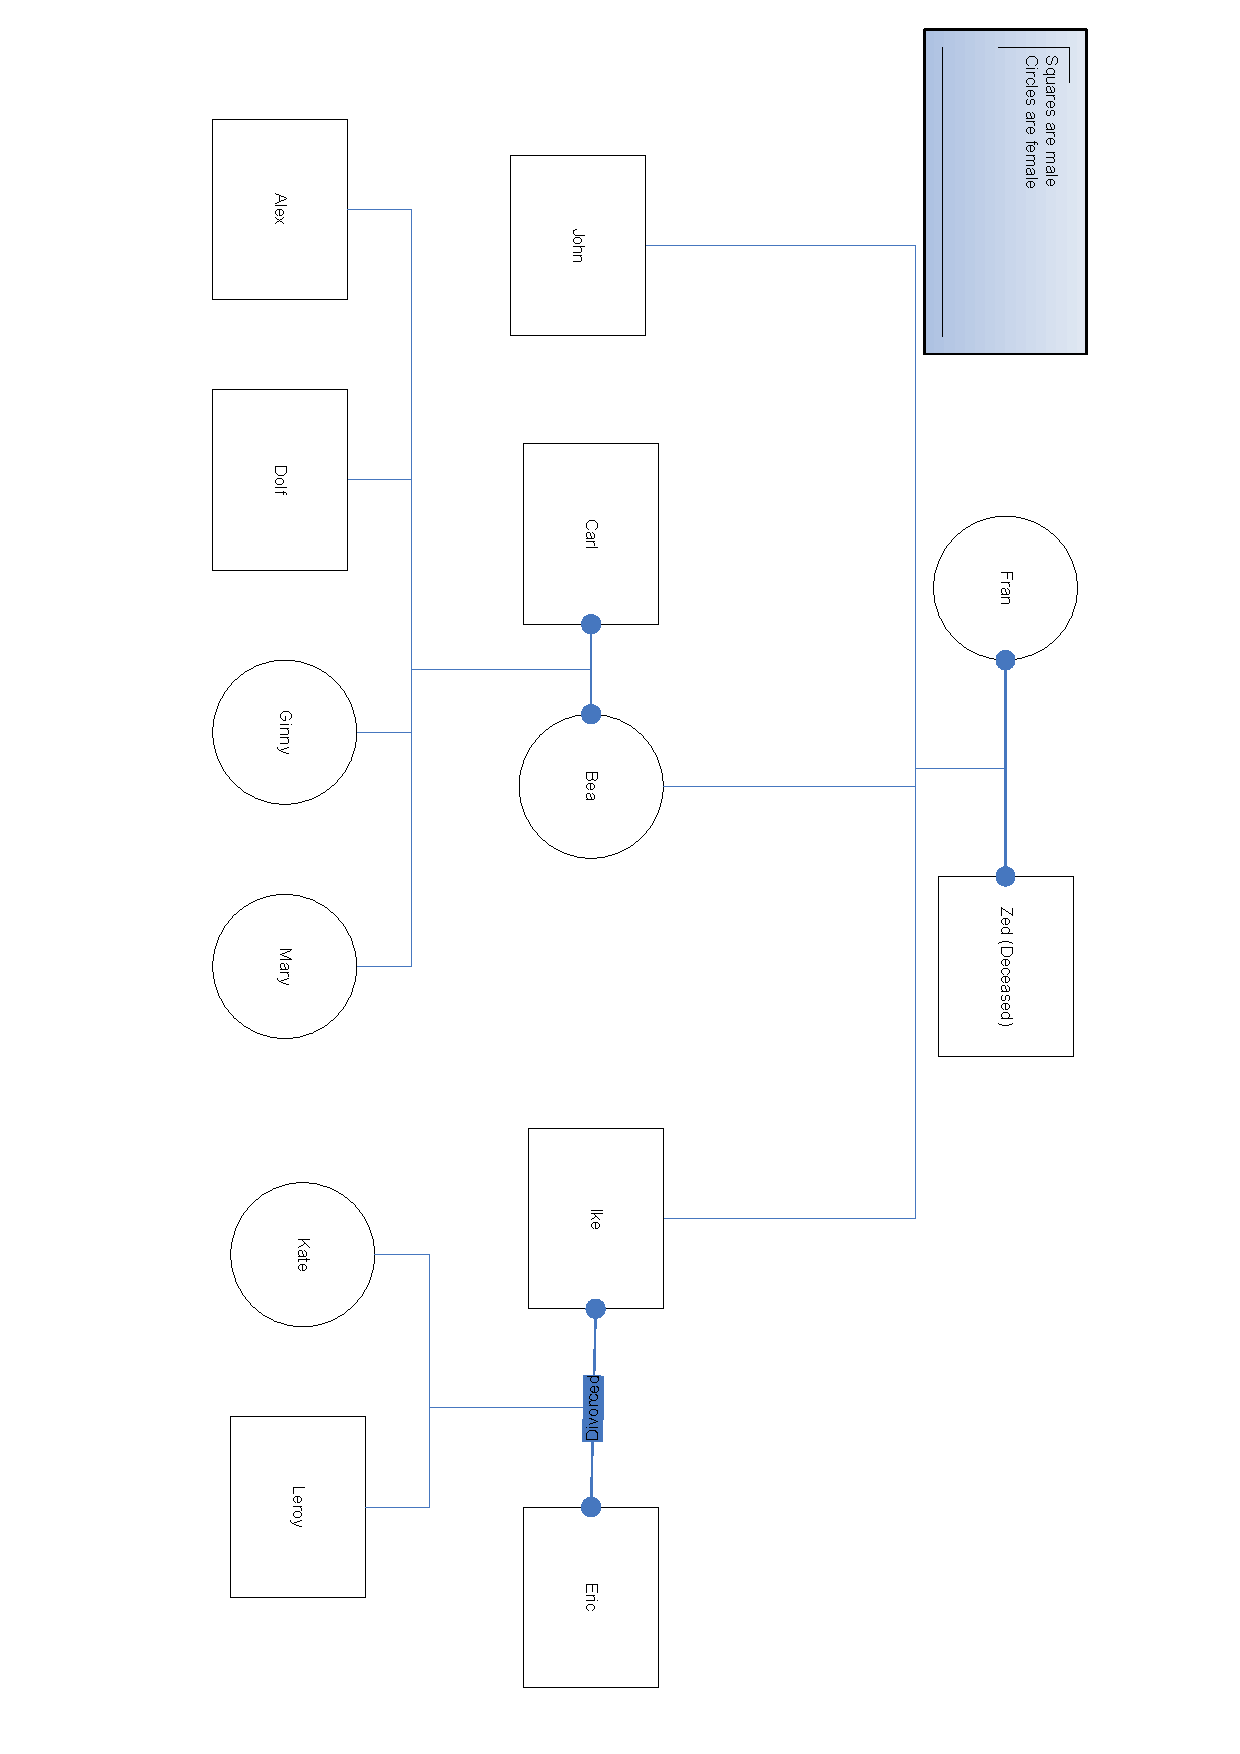
\includegraphics[width=1.3\textwidth]{Familytree.pdf}\\
\caption{Family Tree}\label{fig:famtree}
\end{figure}

\subsubsection*{a.}
The knowledge base for the extended families can be found in the file as2part3a.clp. The family tree can be found in Figure \ref{fig:famtree}. Squares are male, circles are female, connected figures using lines with 2 dots on both sides are spouses, figures that are connected from the spouse relation and are below those spouses, are children from that relation. So for example: Carl is married to Bea, and have 4 children, namely Alex, Dolf, Ginny and Mary. The unreadable up-side down text denotes that the two Ike and Eric are divorced.

The obvious choice for representing people is to use a template. The properties I have defined for a person are: name, gender, age, a possible spouse, and possibly some children. I have chosen for this representation because being a mother, father, sister, brother, husband or wife can be derived from these few properties. Furthermore, because of this representation, we can add a person pretty quickly to the database, because we do not have to manually redefine a lot of properties or relationships that already existed. To add a new child, we would only need to add a new person fact, and add the person to the children list of the two parents. 

The interpretations of these relations are as follows: the mother(x y) relation is interpreted as: x is the mother of y. For the other relations you can replace the name mother for the names of the other relations. The number of individuals added to the knowledge base is 12, all a child of someone, or married to someone (so they have at least one relation). 

\paragraph{Usage:}
To add an additional member to the family one should assert it as a fact. An example is: (assert (person (name piet) (gender male) (age 50) (spouse mary) (children jan henk klaas))). The fields spouse and children are optional. 

Properties can be changed by retracting a fact, by retracting it by it's fact number. Below is an example of a fact list:
\begin{Verbatim}[fontsize=\scriptsize]
==> f-1     (person (name Alex) (gender male) (age 17) (spouse none) (children))
==> f-2     (person (name Bea) (gender female) (age 43) (spouse Carl) (children Alex Dolf Ginny Mary))
==> f-3     (person (name Carl) (gender male) (age 41) (spouse Bea) (children Alex Dolf Ginny Mary))
==> f-4     (person (name Dolf) (gender male) (age 8) (spouse none) (children))
==> f-5     (person (name Eric) (gender male) (age 50) (spouse none) (children Kate Leroy))
==> f-6     (person (name Fran) (gender female) (age 90) (spouse none) (children Bea Ike John))
==> f-7     (person (name Ginny) (gender female) (age 13) (spouse none) (children))
==> f-8     (person (name Ike) (gender male) (age 28) (spouse none) (children Kate Leroy))
==> f-9     (person (name John) (gender male) (age 43) (spouse none) (children))
==> f-10    (person (name Kate) (gender female) (age 6) (spouse none) (children))
==> f-11    (person (name Leroy) (gender male) (age 8) (spouse none) (children))
==> f-12    (person (name Mary) (gender female) (age 30) (spouse none) (children))
\end{Verbatim}
If you would want to change the properties of Alex, for example by making him one year older, you should first issue the command to retract the fact asserting him as a person: (retract 1). Which would remove Alex from the database. One can now add Alex to the database again by using our previous approach: (assert (person (name Alex) (gender male) (age 18))). So now we've removed and added Alex to the database with a cganged age.

Relations most of the times are not specified explicitly, but can be inferred from the properties of a person. So to add a certain relation the best thing to is to add or change a person in the database by using the previous approaches and then using run again. The new relations are then automatically inferred. If one would one to remove or change relations, one should remove the facts from the database that should be changed/removed, change the persons and then rerunning the program. Below are the facts and derived facts from starting the program:
\begin{Verbatim}[fontsize=\scriptsize]
CLIPS> (load as2part3a.clp)
Defining deftemplate: person
Defining deffacts: starting-persons
Defining defrule: der_mother +j+j
Defining defrule: der_father =j+j
Defining defrule: der_sister =j+j+j
Defining defrule: der_brother =j+j+j
Defining defrule: der_husband +j
Defining defrule: der_wife +j
TRUE
CLIPS> (reset)
==> f-0     (initial-fact)
==> f-1     (person (name Alex) (gender male) (age 17) (spouse none) (children))
==> f-2     (person (name Bea) (gender female) (age 43) (spouse Carl) (children Alex Dolf Ginny Mary))
==> f-3     (person (name Carl) (gender male) (age 41) (spouse Bea) (children Alex Dolf Ginny Mary))
==> f-4     (person (name Dolf) (gender male) (age 8) (spouse none) (children))
==> f-5     (person (name Eric) (gender male) (age 50) (spouse none) (children Kate Leroy))
==> f-6     (person (name Fran) (gender female) (age 90) (spouse none) (children Bea Ike John))
==> f-7     (person (name Ginny) (gender female) (age 13) (spouse none) (children))
==> f-8     (person (name Ike) (gender male) (age 28) (spouse none) (children Kate Leroy))
==> f-9     (person (name John) (gender male) (age 43) (spouse none) (children))
==> f-10    (person (name Kate) (gender female) (age 6) (spouse none) (children))
==> f-11    (person (name Leroy) (gender male) (age 8) (spouse none) (children))
==> f-12    (person (name Mary) (gender female) (age 30) (spouse none) (children))
CLIPS> (run)
==> f-13    (mother Bea Mary)
==> f-14    (father Carl Mary)
==> f-15    (sister Ginny Mary)
==> f-16    (brother Dolf Mary)
==> f-17    (brother Alex Mary)
==> f-18    (sister Mary Alex)
==> f-19    (sister Mary Dolf)
==> f-20    (sister Mary Ginny)
==> f-21    (father Ike Leroy)
==> f-22    (father Eric Leroy)
==> f-23    (sister Kate Leroy)
==> f-24    (brother Leroy Kate)
==> f-25    (father Ike Kate)
==> f-26    (father Eric Kate)
==> f-27    (mother Fran John)
==> f-28    (sister Bea John)
==> f-29    (brother Ike John)
==> f-30    (brother John Bea)
==> f-31    (brother John Ike)
==> f-32    (mother Fran Ike)
==> f-33    (sister Bea Ike)
==> f-34    (brother Ike Bea)
==> f-35    (mother Bea Ginny)
==> f-36    (father Carl Ginny)
==> f-37    (brother Dolf Ginny)
==> f-38    (brother Alex Ginny)
==> f-39    (sister Ginny Alex)
==> f-40    (sister Ginny Dolf)
==> f-41    (mother Fran Bea)
==> f-42    (mother Bea Dolf)
==> f-43    (father Carl Dolf)
==> f-44    (brother Alex Dolf)
==> f-45    (brother Dolf Alex)
==> f-46    (father Carl Alex)
==> f-47    (husband Carl Bea)
==> f-48    (mother Bea Alex)
==> f-49    (wife Bea Carl)
\end{Verbatim}
If we now would want to add the fact that Carl and Bea also had Ike as a child we would progress as follows. First we retract redefine the persons that are involved, as we've done before. So we retract both fact 2 and 3. Then we redefine them with the added children by using: (assert (person (name Bea) (gender female) (age 43) (spouse Carl) (children Alex Dolf Ginny Ike Mary)) (person (name Carl) (gender male) (age 41) (spouse Bea) (children Alex Dolf Ginny Ike Mary))). We run the inference process, and the new relations are automatically added. 
\begin{Verbatim}[fontsize=\scriptsize]
CLIPS> (retract 2 3)
<== f-2     (person (name Bea) (gender female) (age 43) (spouse Carl) (children Alex Dolf Ginny Mary))
<== f-3     (person (name Carl) (gender male) (age 41) (spouse Bea) (children Alex Dolf Ginny Mary))
CLIPS> (assert (person (name Bea) (gender female) (age 43) (spouse Carl) (children Alex Dolf Ginny Ike Mary)) 
               (person (name Carl) (gender male) (age 41) (spouse Bea) (children Alex Dolf Ginny Ike Mary)))
==> f-50    (person (name Bea) (gender female) (age 43) (spouse Carl) (children Alex Dolf Ginny Ike Mary))
==> f-51    (person (name Carl) (gender male) (age 41) (spouse Bea) (children Alex Dolf Ginny Ike Mary))
<Fact-51>
CLIPS> (run)
==> f-52    (sister Ginny Ike)
==> f-53    (sister Mary Ike)
==> f-54    (brother Ike Ginny)
==> f-55    (brother Ike Dolf)
==> f-56    (brother Ike Alex)
==> f-57    (brother Alex Ike)
==> f-58    (brother Dolf Ike)
==> f-59    (brother Ike Mary)
==> f-60    (father Carl Ike)
==> f-61    (mother Bea Ike)
\end{Verbatim}
To process something like a divorce the relations stating that the two are married should be retracted, the persons should be modified to reflect they have no spouse anymore, and the inference process can be run if necessary.

Now to answer queries a rule printing the answer to the query should be defined. So if we would for example want to know the age of John we would define a rule like this:
\begin{Verbatim}[fontsize=\scriptsize]
CLIPS> (defrule john_age (person (name John) (age ?ag)) => (printout t "The age of John is: " ?ag crlf))
CLIPS> (run)
The age of John is: 43
\end{Verbatim}
So we should match on a person with a specific name, take the wanted attribute as a variable and then print that. 

To list all properties of an entity we can do something similar. So if we wanted to know attributes of Leroy's father we would first match on the person (and his name Leroy), get the needed name from the father relation. After that we can get the attributes from that father the same way as we just did in the previous example. Below is an example that gets the data of the father of leroy. In the example below I deliberately use a person with two fathers to show it also works generally. 
\begin{Verbatim}[fontsize=\scriptsize]
CLIPS> (defrule leroy_father 
 (person (name Leroy)) 
 (father ?fa Leroy) 
 (person (name ?nm) 
         (gender ?m) ;this should of course be male 
         (age ?ag) 
         (spouse ?sp) 
         (children $?ch) 
 ) 
 (test (eq ?fa ?nm)) 
=>  
 (printout t "The name of the father of John is: " ?nm crlf 
             "The gender of the father of John is: " ?m crlf 
             "The age of the father of John is: " ?ag crlf 
             "The spouse of the father of John is: " ?sp crlf 
             "The children of the father of John is: " $?ch crlf 
 ) 
)
CLIPS> (run)
The name of the father of John is: Eric
The gender of the father of John is: male
The age of the father of John is: 50
The spouse of the father of John is: none
The children of the father of John is: (Kate Leroy)
The name of the father of John is: Ike
The gender of the father of John is: male
The age of the father of John is: 28
The spouse of the father of John is: none
The children of the father of John is: (Kate Leroy)
\end{Verbatim}
To identify an individual with certain properties we can almost use the same method as we used to query about properties from one person. But now we remove the test on the name and add a test for a specific attribute for those persons. As an example we list the individuals with an age lower than 40. See below for an example run:
\begin{Verbatim}[fontsize=\scriptsize]
CLIPS> (defrule age_less_than_40 
 (person (name ?nm) 
         (gender ?m) 
         (age ?ag) 
         (spouse ?sp) 
         (children $?ch) 
 ) 
 (test (< ?ag 40)) ;the important part, the test for a certain property! 
=>  
 (printout t "The name of the person is: " ?nm crlf 
             "The gender of the person is: " ?m crlf 
             "The age of the person is: " ?ag crlf 
             "The spouse of the person is: " ?sp crlf 
             "The children of the person are: " $?ch crlf 
 ) 
)
CLIPS> (run)
The name of the person is: Mary
The gender of the person is: female
The age of the person is: 30
The spouse of the person is: none
The children of the person are: ()
The name of the person is: Leroy
The gender of the person is: male
The age of the person is: 8
The spouse of the person is: none
The children of the person are: ()
The name of the person is: Kate
The gender of the person is: female
The age of the person is: 6
The spouse of the person is: none
The children of the person are: ()
The name of the person is: Ike
The gender of the person is: male
The age of the person is: 28
The spouse of the person is: none
The children of the person are: (Kate Leroy)
The name of the person is: Ginny
The gender of the person is: female
The age of the person is: 13
The spouse of the person is: none
The children of the person are: ()
The name of the person is: Dolf
The gender of the person is: male
The age of the person is: 8
The spouse of the person is: none
The children of the person are: ()
The name of the person is: Alex
The gender of the person is: male
The age of the person is: 17
The spouse of the person is: none
The children of the person are: ()
\end{Verbatim}
And finally to answer queries about relationships are very easy now we already know how to query persons. To for example find the brothers of Ginny we do the following:

\begin{Verbatim}[fontsize=\scriptsize]
CLIPS> (defrule ginny_brothers  
 (brother ?nm Ginny) ;?nm is the brother of Ginny 
=> 
 (printout t "The name of the brother of Ginny is: " ?nm crlf) 
)
CLIPS> (run)
The name of the brother of Ginny is: Alex
The name of the brother of Ginny is: Dolf
\end{Verbatim}
This concludes the description of how to get facts out of the knowledge base.

\subsubsection*{b.}
The knowledge base defined in a. and extended with new relationships can be found in the file as2part3b.clp. A parent can be derived by just making every father and mother of a child a parent of that child. (I interpreted parent as a relation between parent and child.) A sibling can similarly be generalized from the brother and sister relations. 

For the cousin relation I only consider first cousins, but this can of course be generalized. (A first cousin is a child from a sibling from one of your parents.) So the rule takes a parent of for instance John, the sibling from the parent of John, and then relates the child from that sibling with John with the cousin relation. 

For in-laws I take the definition that an in-law is either a wife or a husband. So inferring this as a rule is similar to the deriving of a parent and sibling.

A grandfather is male that has a child that has a child. The rule can therefore be constructed by making a relation by finding a father. Then checking if that father's child is a parent, and then connecting that child with the father with the grandfather relation. The generalizing to grandparent is again obvious and similar to the parent a sibling rule. 

An uncle or aunt is a relation from a person to a child of his sibling. So for a child an uncle is a brother or brother-in-law of his parent. So the rule for uncles and aunts takes a parent and his/her children, and connects all the siblings with these children with the uncle/aunt relation.


\subsection*{4: Search}
\subsubsection*{a.}
The initial state is Arad, and the goal state is Bucharest. The set of states in the search space is infinite. One path with infinite states for example is $Arad \rightarrow Sibiu \rightarrow Oradea \rightarrow Zerind \rightarrow Arad \rightarrow Sibiu...$. 
The complete set of cities is C = \{Arad, Bucharest, Craiova, Dobreta, Eforie, Fagaras, Giurgiu, Hirsova, Iasi, Lugoj, Mehadia, Neamt, Oradea, Pitesti, Rimnicu Vilcea, Sibiu, Timisoara, Urziceni, Vaslui, Zerind\}. But not all these cities can be reached. The cities right from Bucharest (in the picture) can not ever be visited with one of the search algoritms. A goal test will end the search in Bucharest. The number of different states therefore is the collection C minus the unreachables cities U = \{Eforie, Hirsova, Iasi, Neamt, Urziceni, Vaslui\}. Thus the number of different states us $|C \backslash U| = |$\{Arad, Bucharest, Craiova, Dobreta, Fagaras, Giurgiu, Lugoj, Mehadia, Oradea, Pitesti, Rimnicu Vilcea, Sibiu, Timisoara, Zerind\}$| = 14$. \\
After simplifying the problem in b (see Figure \ref{fig:searchtreesimple}), we only have 16 states, of which only 5 are unique.
\subsubsection*{b.}
After simplifying the state space we get the following picture.\\
\begin{figure}[htp]
\centering
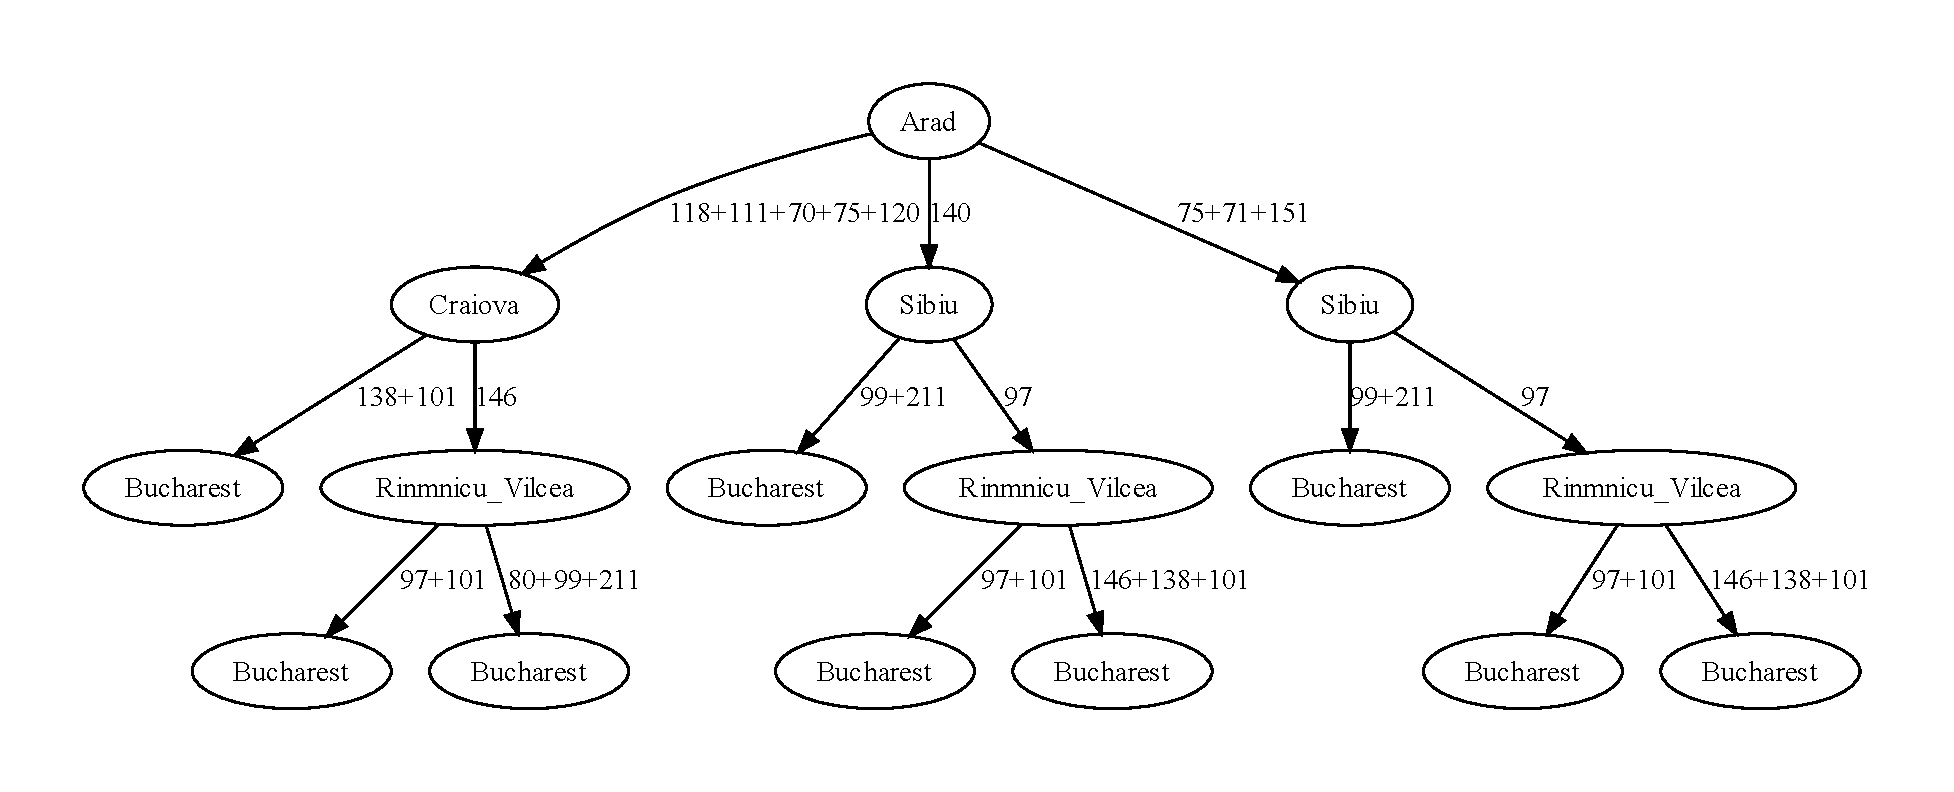
\includegraphics[width=1.3\textwidth]{notsummed.pdf}\\
\caption{Search tree}\label{fig:searchtree}
\end{figure}\\
This can again be simplified into:\\
\begin{figure}[htp]
\centering
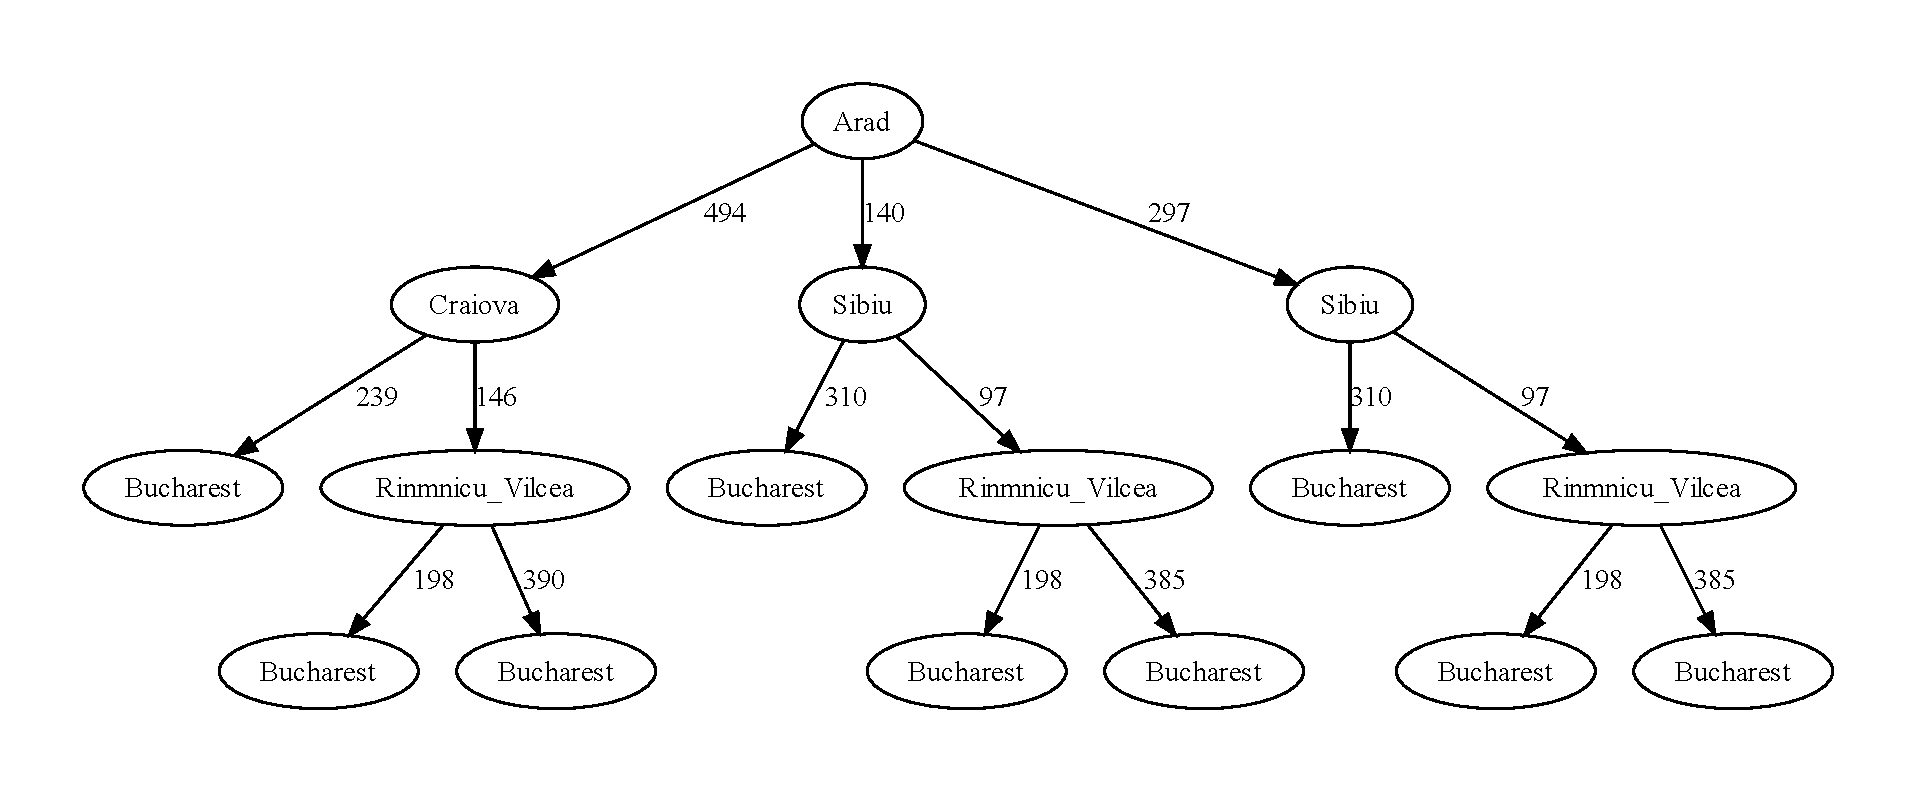
\includegraphics[width=1.3\textwidth]{summed.pdf}\\
\caption{Simplified search tree}\label{fig:searchtreesimple}
\end{figure}\\
\subsubsection*{c.}

\paragraph*{I.}
Assuming depth first search takes nodes from left to right the nodes expanded will be: $Arad \rightarrow Craiova \rightarrow Bucharest$. This expansion of nodes also is the path to the solution. The total path cost of this solution is: $494 + 239 = 733$.

\paragraph*{II.}
Again assuming that order of expansion is from left to right the nodes expanded will be: $Arad \rightarrow Craiova \rightarrow Sibiu \rightarrow Sibiu \rightarrow Bucharest$. The path taken is ultimately the same as with depth first search, namely $Arad \rightarrow Craiova \rightarrow Bucharest$, with a total path cost of $494 + 239 = 733$.

\paragraph*{III.}
Now we also have to keep the straight line distance in account when expanding nodes. First we decorate the previous Figure \ref{fig:searchtreesimple} with straight line distances and traveled distance to make expansion easier. \\
\begin{figure}[htp]
\centering
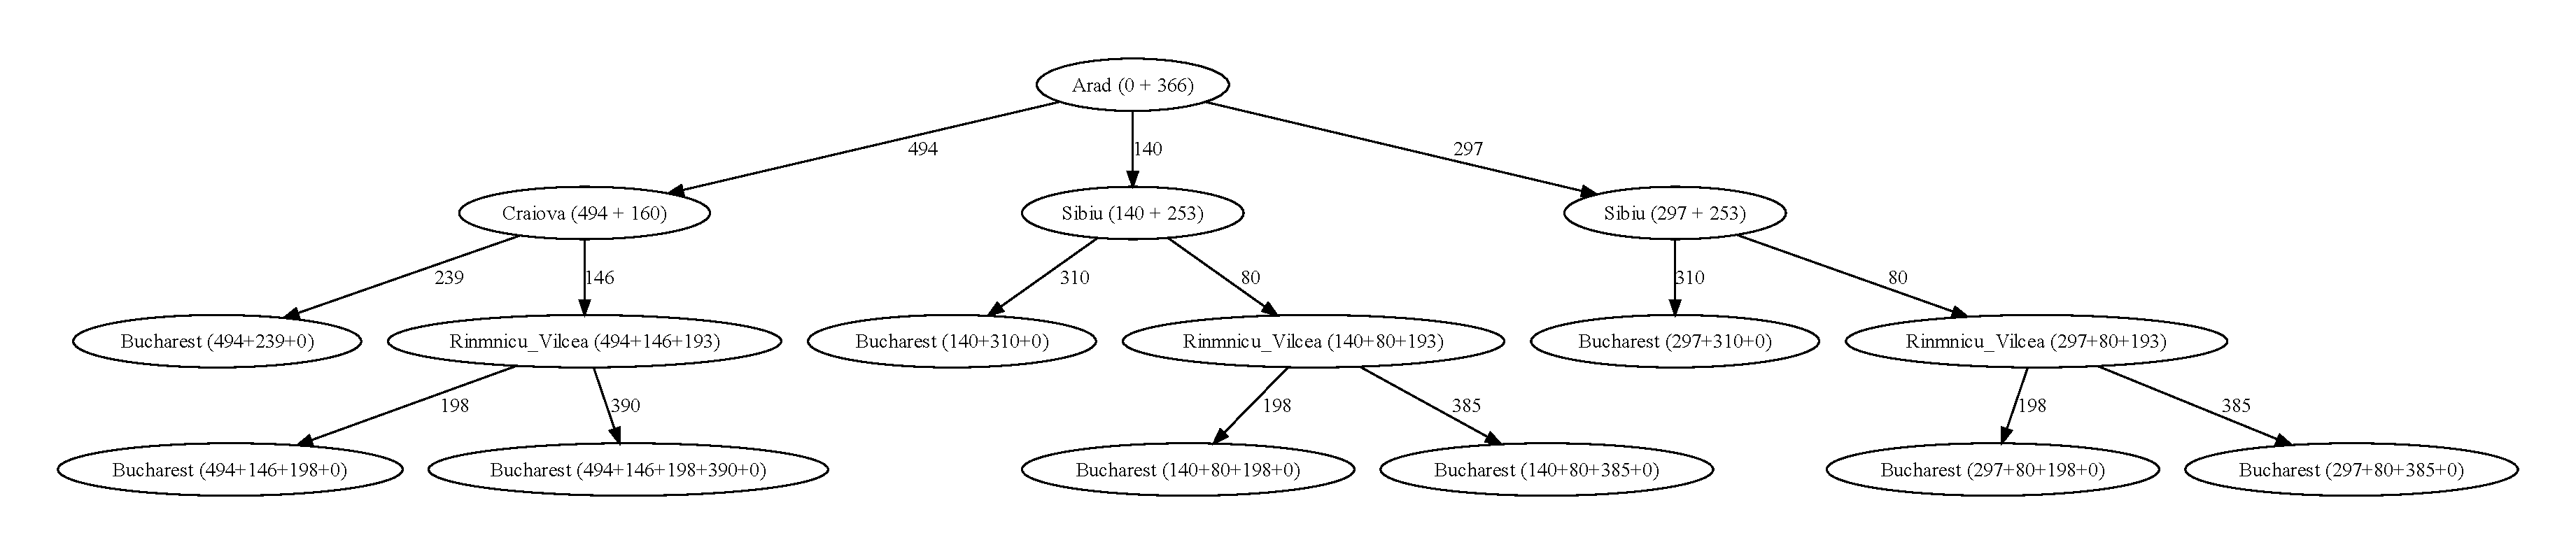
\includegraphics[width=1.3\textwidth]{notsummedstraightline.pdf}\\
\caption{Search tree with straight line distances}\label{fig:searchtree2}
\end{figure}\\
This is again simplified in Figure \ref{fig:searchtree2simple}.
\begin{figure}[htp]
\centering
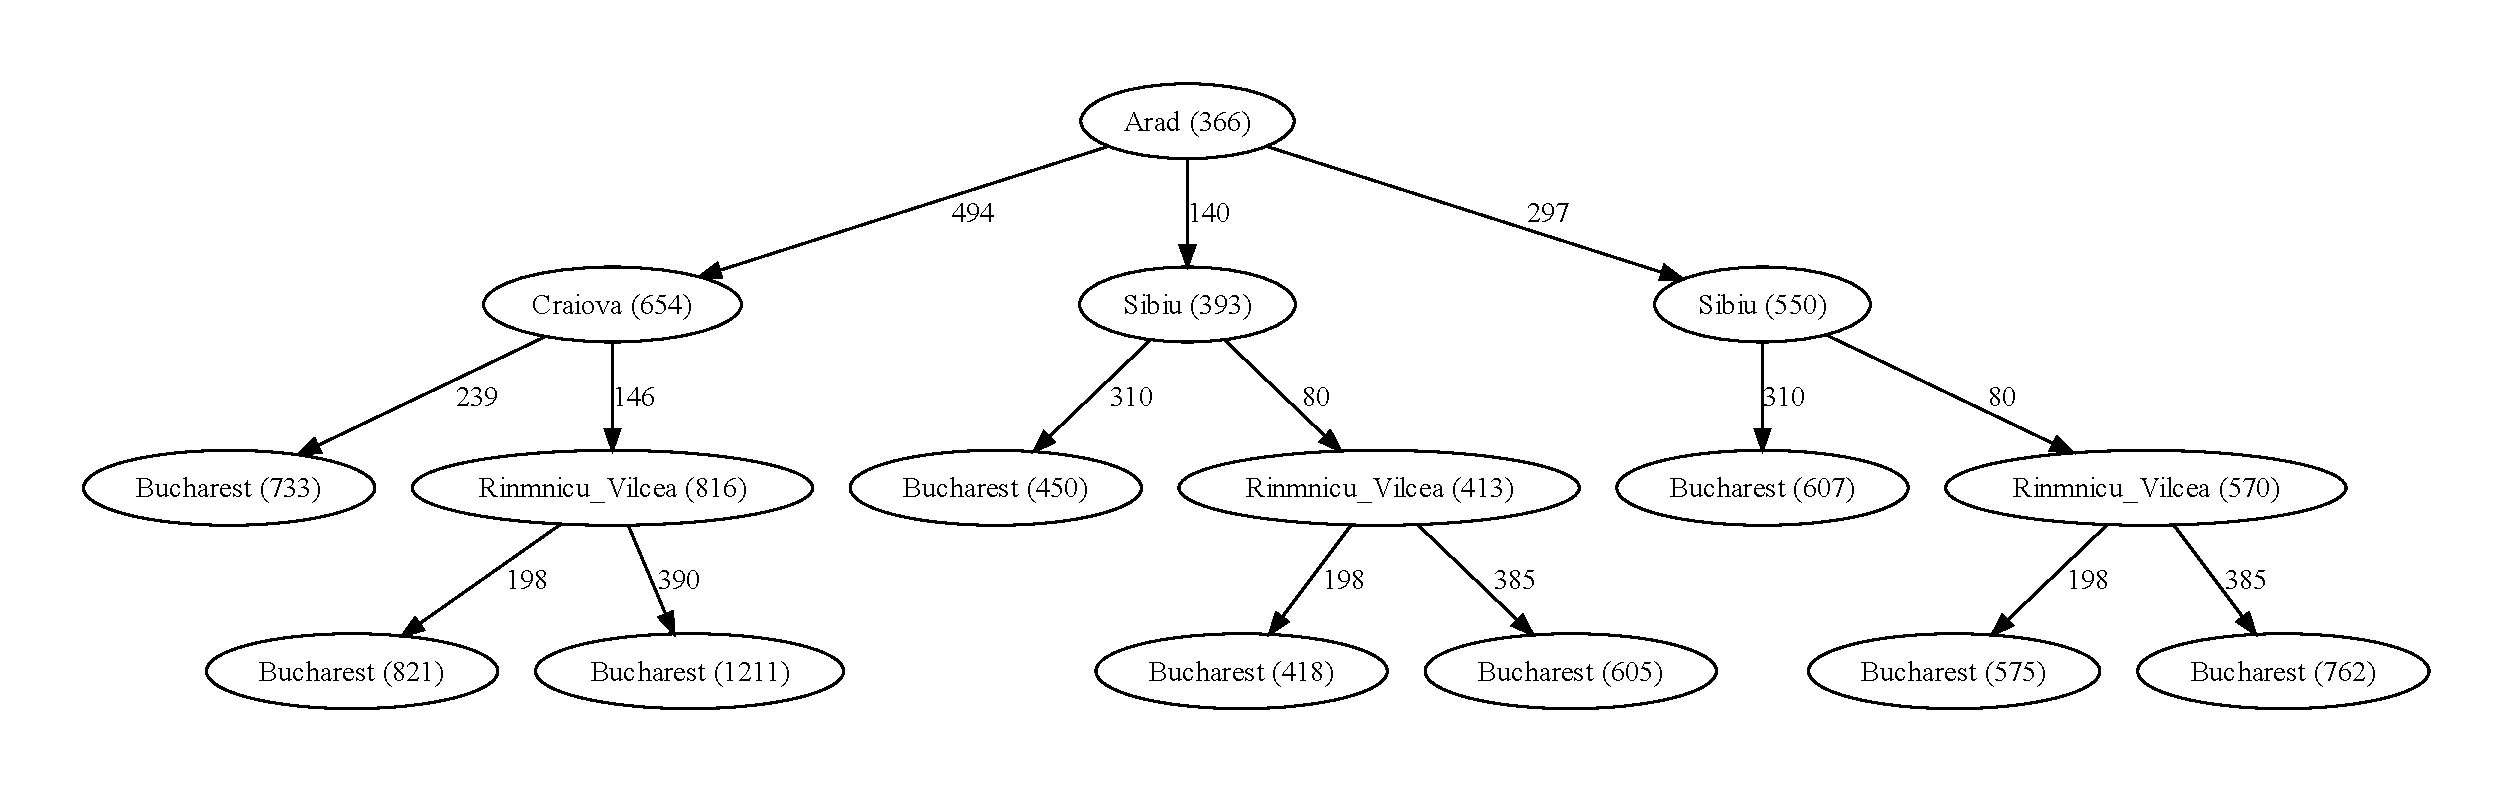
\includegraphics[width=1.3\textwidth]{summedstraightline.pdf}\\
\caption{Simplified search tree with straight line distances}\label{fig:searchtree2simple}
\end{figure}
The first node to be expanded is of course Arad. After that the node with the lowest cost that has not been expanded yet will be expanded. In this case this is pretty straightforward as the expanded nodes will be: $Arad \rightarrow Sibiu \rightarrow Rinmicu\_Vilcea \rightarrow Bucharest$. The path taken takes a total path cost of $140 + 80 + 198 = 418$. Because A* search is optimal, this is also the optimal path. 

\subsubsection*{d.}
Depth-first search is incomplete if a the search tree contains infinite paths. This means that for a route finding problem, such as the unsimplified version of the previous problem, a depth-first search would continue infinitely down a path without ever finding a solution. Furthermore, depth-first search and breadth-first search are both not optimal (the latter is only optimal at equal step costs for every path). Thus depth-first and breadth first search do not return the best solution. Breadth-first also uses a high amount of space in comparison to depth first and A* search. Breadth first search keeps every expanded node in memory, which amounts to a very high usage of space. The amount of time taken for both depth-first and breadth-first search is also quite large, because both algorithms search uninformed and thus blindly. Without guidelines guiding the search the amount of time needed to travel the search can be quite large.

A* search is optimal, given that the heuristic is both admissible and consistent. This is already a big improvement over depth-first and breadth-first search. Furthermore, A* search uses at most as much memory as breadth first search(in the case all paths have the same cost), but probably less. The memory usage of A* search is less space efficient than depth-first search though. Time consumption for A* search depends a lot on the heuristic, but given a reasonable heuristic the time taken to solve the problem is quite less than the other two search techniques. And finally, A* is complete(, in contrast to depth-first search).

Thus the algorithm to use for route-finding problems would be A* search.



\end{document}